\subsection{Problem and Motivation}

\begin{frame} \frametitle{Problem}
  \begin{itemize}
    \item Problem: maintain a global timescale through the system 
	\begin{figure}
	\centering
	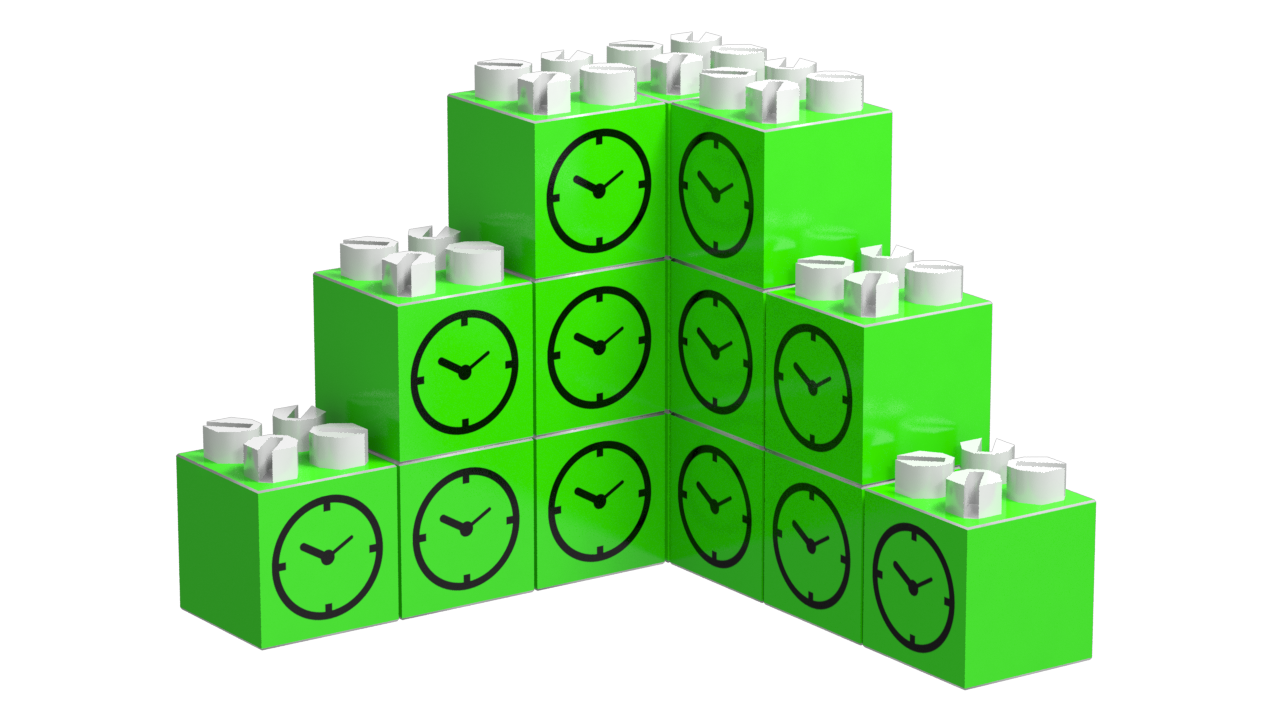
\includegraphics[height=0.325\paperheight]{fig/synchronization/clock-bb-illustration.png}
	\end{figure}
    \item Challenges:
      \begin{itemize}
      \item Imperfect hardware clocks (clock drift, skew, offset and noise)
      \item Handling communication delays
      \end{itemize}
 \end{itemize}
\end{frame}

\noLogo{
\begin{frame} \frametitle{Motivation}

Distributed coordination (e.g., distributed bitmap scroller)

\begin{center}	
	\begin{columns}[c]
		\begin{column}{.5\textwidth}
		\centering
		\href{run:videos/31-scroller-goal.avi?autostart&loop}{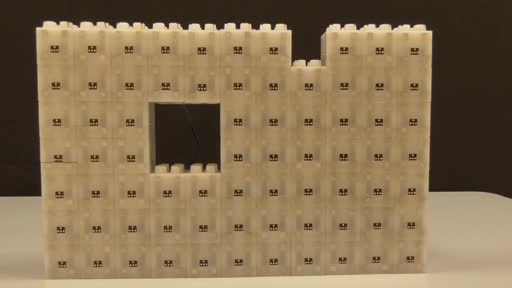
\includegraphics[width=0.95\linewidth]{videos/31-scroller-goal.jpg}}
		\end{column}
		\begin{column}{.5\textwidth}
		\centering			
		72-Blinky-Blocks scroller synchronized with our protocol (MRTP)
		\end{column}
	\end{columns}
\end{center}

Unsynchronized scroller:
\begin{center}	
\begin{columns}[c]
	\begin{column}{.33\textwidth}
		\centering
		Start:\\
		\href{run:videos/31-unsync1.avi?autostart&loop&start=1}{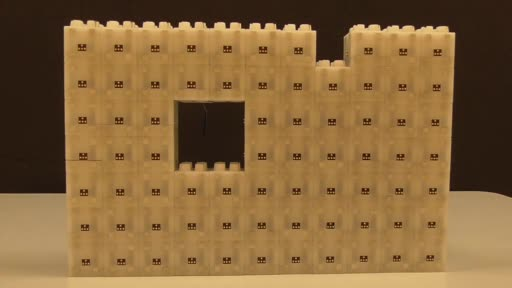
\includegraphics[width=0.9\linewidth]{videos/31-unsync1.jpg}}
	\end{column}
	\begin{column}{.33\textwidth}
		\centering
		1min20:\\
		\href{run:videos/31-unsync2.avi?autostart&loop}{
\includegraphics[width=0.95\linewidth]{videos/31-unsync2.jpg}}
	\end{column}  
	\begin{column}{.33\textwidth}
		\centering
		20min:\\
		\href{run:videos/31-unsync3.avi?autostart&loop}{
\includegraphics[width=0.95\linewidth]{videos/31-unsync3.jpg}}
	\end{column} 
\end{columns}
\end{center}
\vspace{-0.35cm}
\remark{This application requires a global timescale}
\end{frame}
}

\subsection{Assumptions}

\begin{frame}\frametitle{Assumptions}

Illustrated on the Blinky Blocks modular robot, but suitable for networked embedded devices with:

	\begin{itemize}
		%\item Non-anonymous (unique identifiers used for leader election)
    	\item Local clocks
    		\begin{itemize}
    			\item Nearly identical precision/resolution (potentially poor)
    				\begin{itemize}
    					\item Blinky Blocks: 1\% precision, 1 ms resolution
    				\end{itemize}
    		%	\item Quasi-linear skew
    		\end{itemize}
    	\item Network
    	    \begin{itemize}
    	    	%\item Undirected and unweighted 
    	    	\item Neighbor-to-Neighbor communications
    	    	\item Potentially: large network size and large diameter
    	    	\item Fairly stable
    	    	%\item Low-level timestamping mechanism
    	    \end{itemize}
    \end{itemize}

\begin{center}
\begin{columns}[c]
	\begin{column}{.5\textwidth}
		\centering
		Split:\\
		\href{run:videos/32-split.avi?autostart&loop}{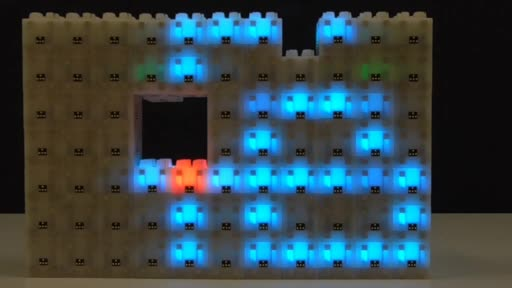
\includegraphics[width=0.9\linewidth]{videos/32-split.jpg}}
	\end{column}
	\begin{column}{.5\textwidth}
		\centering
		Merge (after 2 hours):\\
		\href{run:videos/32-merge.avi?autostart&loop}{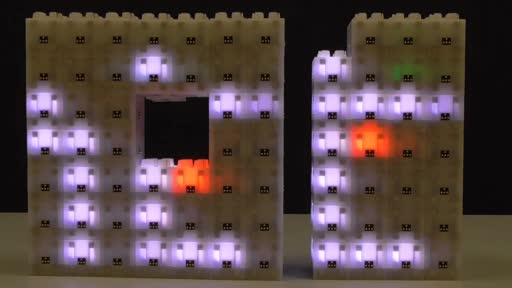
\includegraphics[width=0.9\linewidth]{videos/32-merge.jpg}}		
	\end{column} 
\end{columns}
\end{center}

\end{frame}

\subsection{Related Work}

\noLogo{
\newcommand{\lenMinusOne}{0.08\linewidth}
\newcommand{\lenZero}{0.08\linewidth}
\newcommand{\lenOne}{0.12\linewidth}
\newcommand{\lenTwo}{0.16\linewidth}
\newcommand{\lenThree}{0.20\linewidth}
\newcommand{\lenFour}{0.15\linewidth}
\begin{frame} %[shrink=2]
  \frametitle{Related Works}

\vspace{-0.25cm}
\tiny
\begin{center}
	\begin{tabular}{|C{\lenFour}|C{\lenZero}|C{\lenTwo}|C{\lenMinusOne}|C{\lenThree}|C{\lenOne}|}
	\hline
	Name &  Domain & Architecture & Infrastructure & Synchronization Technique & Clock Skew Compensation\\
	\hline
	NTP \cite{mills1991internet} & \multirow{4}{\linewidth}{\centering Computer Networks} & Master/Slave Master(s): pre-configured & \multirow{4}{\linewidth}{\centering Tree} & (Multi-hop) round-trip messages with frame-level timestamps and statistics & Phase/frequency locked loops \\
	\cline{1-1}
	\cline{3-3}
	\cline{5-6}
	PTP \cite{ptp2008} & & Master/slave Master: best clock & & Round-trip with low-level timestamps and per-hop delay compensation & \\
	\hline
	RBS \cite{elson2002fine} & \multirow{15}{\linewidth}{\centering Sensor Networks} & Master/Slave & Clustering  & Reference broadcast  & \multirow{15}{\linewidth}{\centering Linear model} \\
	\cline{1-1}
	\cline{3-5}	
	ATS [Schenato et al., 2011] &  & \multirow{4}{\linewidth}{\centering Fully distributed} & \multirow{4}{\linewidth}{\centering /} & Average-based consensus. Byte-level timestamps &  \\
	% \cite{schenato2011average}
	\cline{1-1}
	\cline{5-5}
	MTS \cite{he2014time,he2014study} &  &  & & Extremum-value based consensus. Byte-level timestamps & \\
	\cline{1-1}
	\cline{3-5}
	TPSN + MLE \cite{leng2010clock} &  & Master/slave & Tree & Recursive per-hop synchronization. Round- trip with frame-level timestamps and statistics & \\
	\cline{1-1}
	\cline{3-5}
	FTSP \cite{maroti2004flooding} &  & \multirow{5}{\linewidth}{\centering Master/slave Master: minimum-id implicit election} &  \multirow{4}{\linewidth}{\centering /} & Periodic asynchronous broadcasts. Byte-level timestamps and statistics &  \\
	\cline{1-1}
	\cline{5-5}			
	PulseSync \cite{lenzen2015pulsesync} &  & & & Fast flooding using broadcast. Byte-level timestamps & \\
	\hline
	\end{tabular}
\end{center}

\begin{center}
	\begin{tabular}{|C{\lenFour}|C{\lenZero}|C{\lenTwo}|C{\lenMinusOne}|C{\lenThree}|C{\lenOne}|}
	\hline
	Contribution: MRTP  & \textcolor{\remarkColor}{Modular Robotic} & Master/Slave  \textcolor{\remarkColor}{Master: central} & \textcolor{\remarkColor}{Breadth- first} spanning- tree &  Fast recursive per-hop synchronization. \textcolor{\remarkColor}{Compensation comm. delays: best for target system} & Linear model\\
	\hline
	\end{tabular}
\end{center}
\end{frame}
}

\subsection{Contribution: The Modular Robot Time Protocol (MRTP)}

\subsectionOutlineFrame

\subsubsection{Workflow}
\begin{frame} \frametitle{Contribution: The Modular Robot Time Protocol (MRTP)}
\begin{center}
    \begin{columns}[t]
      \begin{column}{.80\textwidth}
		\begin{enumerate}
			\item Initialization
			\begin{enumerate}
			\item Central time master election
			%(e.g., ABC-Center, $k$-BFS SumSweep, PC2LE)
			\item Breadth first spanning-tree construction
			%\item Set all clocks to the maximum global clock
			\end{enumerate}
			\item Periodic synchronization
			\begin{itemize}
				\item Best-suited method to compensate for\\communication delays
				\item Clock skew compensation using linear regression
			\end{itemize}
		\end{enumerate}
      
      ~\\
      $G(t)$: global time, held by the time master\\
      $\tilde{G}(t)$: disseminated estimation of $G(t)$
      
      \end{column}
      \begin{column}{.20\textwidth}
		\begin{figure}
			\centering
			\hspace{-1cm}
			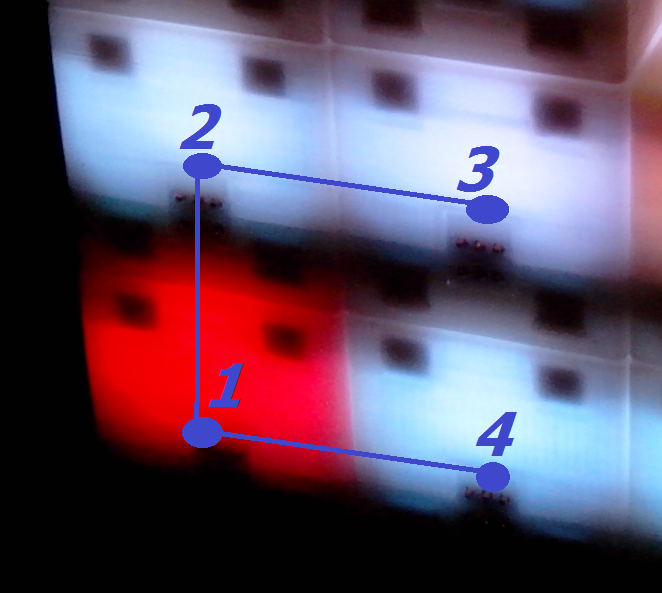
\includegraphics[width=1.25\linewidth]{fig/synchronization/sub-system}\\~\\
			\vspace*{-0.25cm}
			\hspace*{-3cm}
			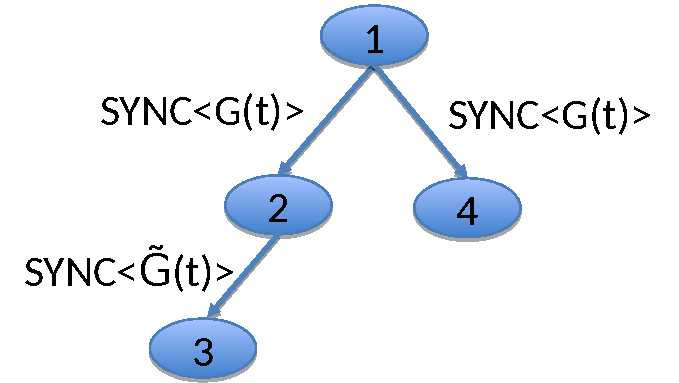
\includegraphics[width=2.3\linewidth]{fig/synchronization/tree}
			\label{fig:sub-system}
		\end{figure}
      \end{column}
  \end{columns}
  \end{center}
\end{frame}

\subsubsection{The Predictive Method to Compensate for Communication Delays}

\begin{frame} \frametitle{The Predictive Method to Compensate for Communication Delays}

\begin{figure}
	\centering
	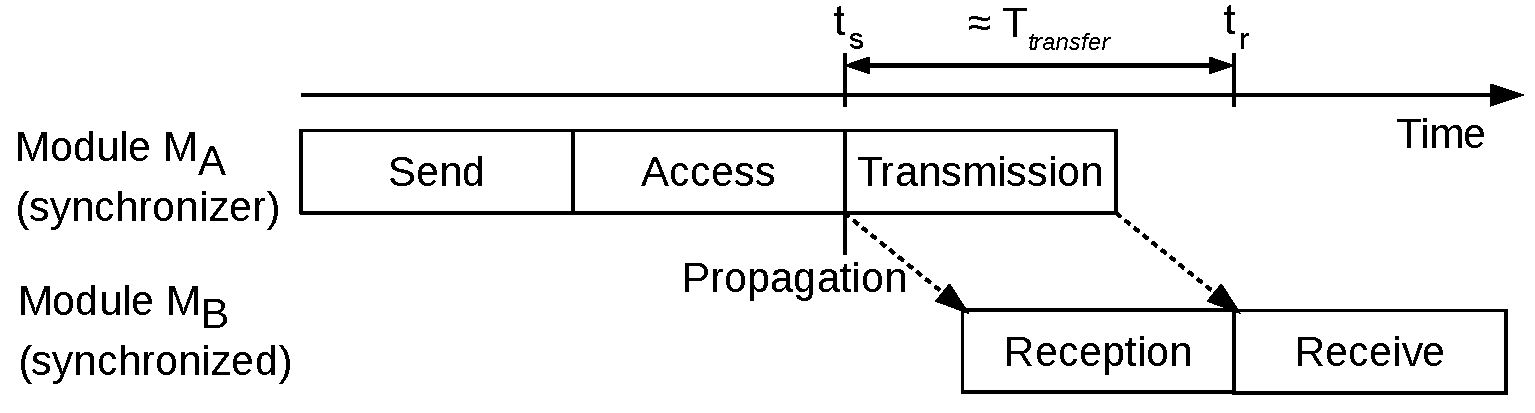
\includegraphics[width=0.75\linewidth]{fig/synchronization/synchronization-timestamp}
	\label{fig:synchronization-timestamp}
\end{figure}

\begin{figure}
	\centering
	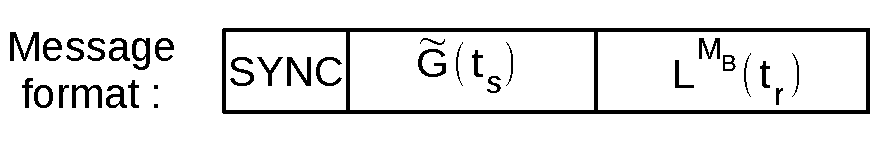
\includegraphics[width=0.5\linewidth]{fig/synchronization/synchronization-message}
	\label{fig:synchronization-message}
\end{figure}

\begin{center}
	\[
	\tilde{G}(t_r) = \tilde{G}(t_s) + T_{transfer}
	\]
	Linear regression on a window of synchronization points $<\tilde{G}(t),L^{M_B}(t)>$
	\[
	G^{M_B}(t) = a^{M_B}(t) * L^{M_B}(t) + b^{M_B}(t)
	%\forall t, \forall t', t \geq t', \ G^{M_B}(t) = max(G^{M_B}(t'),\ a^{M_B}(t)*L^{M_B}(t) + b^{M_B}(t))
	\]
\end{center}

\end{frame}

\subsection{Evaluation}

\subsectionOutlineFrame

\subsubsection{Blinky Blocks: Compensation for Communication Delays?}

\begin{frame}\frametitle{The Blinky Blocks Communication delays}

\begin{center}
	\begin{columns}[c]
		\begin{column}{.50\textwidth}
			\begin{figure}
				\centering
				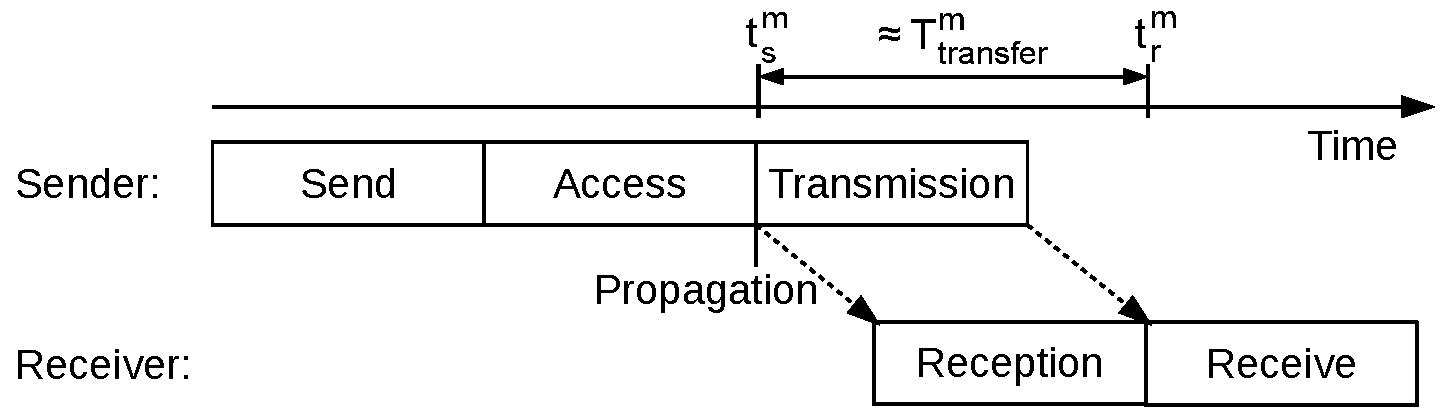
\includegraphics[width=\linewidth]{fig/synchronization/network-delay}
				\label{fig:communication-delays}
			\end{figure}
		\end{column}
		\begin{column}{.50\textwidth}
			\begin{figure}
				\centering
				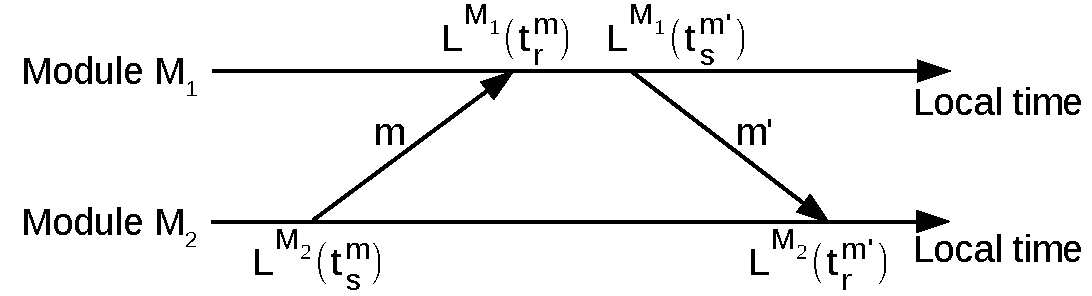
\includegraphics[width=\linewidth]{fig/synchronization/two-way}
				\label{fig:two-way}
			\end{figure}
			
		\end{column}
	\end{columns}
\end{center}

{
	\[ T_{transfer} \approx \frac{(L^{M_2}(t_r^{m'}) - L^{M_2}(t_s^m)) - (L^{M_1}(t_s^{m'})-L^{M_1}(t_r^m))}{2}\]
}

\vspace*{-0.75cm}
\begin{center}
	\begin{columns}[c]
		\begin{column}{.22\textwidth}
			\begin{figure}
				\centering
				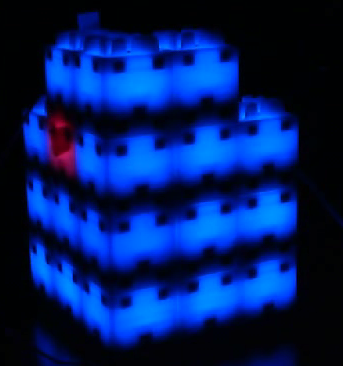
\includegraphics[width=0.75\linewidth]{fig/synchronization/dense}
				\label{fig:system}
			\end{figure}
		\end{column}
		\begin{column}{.53\textwidth}
			\begin{figure}
				\centering
				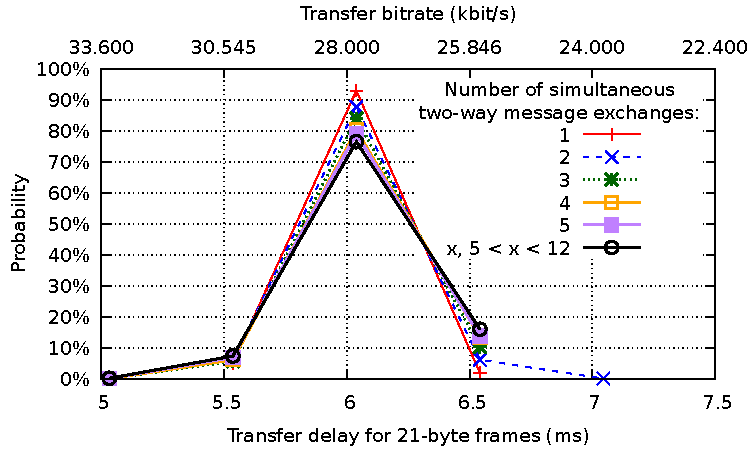
\includegraphics[width=\linewidth]{fig/synchronization/delayNeighborhood}
				\label{fig:transfer-measures}
			\end{figure}
		\end{column}
		\begin{column}{.25\textwidth}	
			300,000 two-way exchanges\\
				~\\$\overline{T_{transfer}} \approx$\\
				 \hspace{1cm} $\frac{\text{frame size}}{28.00}$
		\end{column}
	\end{columns}
	
	\remark{Predictable transfer delays}
\end{center}
\end{frame}

\noLogo{
	\begin{frame} \frametitle{Best Method to Compensate for the Blinky Blocks Communication Delays?}
	
	Methods applicable on the Blinky Blocks
	\begin{itemize}
		\item Predictive (PRED)
		\item Round-Trip Time (RTT): used in TPSN  
		\item Frame Delimiter (FD): used in ATS and MTS
	\end{itemize}
	
	\begin{center}
		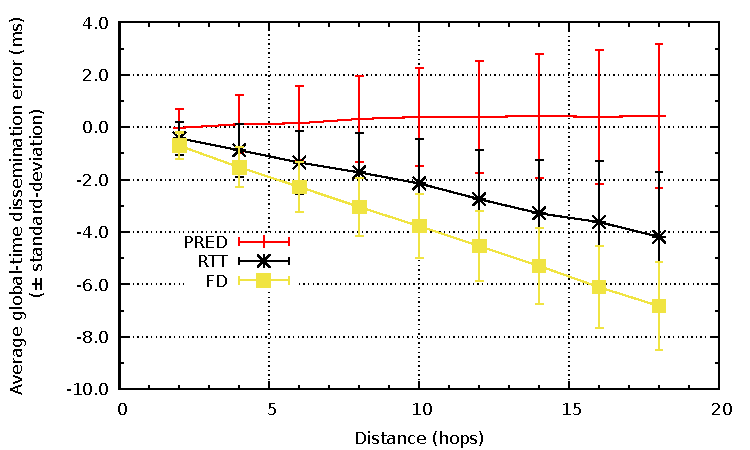
\includegraphics[width=0.6\linewidth]{fig/synchronization/dissemination-error-hw}
		\remark{PRED is the most accurate and uses a single message per hop}
	\end{center}
	\end{frame}
}

\noLogo{
\subsubsection{Hardware Results}

\begin{frame} \frametitle{Synchronizable Radius}
  \centering
  \begin{center}
    \begin{columns}[c]
      \begin{column}{.45\textwidth}
        \centering
        \adjincludegraphics[width=.95\linewidth,valign=t]{fig/synchronization/line1.png}\\
      \end{column}
      \begin{column}{.45\textwidth}
        \centering
        \adjincludegraphics[width=.95\linewidth,valign=t]{fig/synchronization/line2.png}\\
      \end{column}
  \end{columns}
  \end{center}	
  	
  \remark{The time master synchronizes modules in a 27-hop radius to $< 40 ms$}
  \vspace{-1em}
  \begin{center}
  	\begin{columns}[c]
  		\begin{column}{.8\textwidth}
  		\centering
		\remark{Extrapolation: with a central time master, MRTP can synchronize the 27-hop-radius ball system (octahedral shape with 27,775 modules) to $< 40 ms$.}
		\remark{We will use simulations to show it!}
  		\end{column}
  		\begin{column}{.2\textwidth}
  		\centering
  		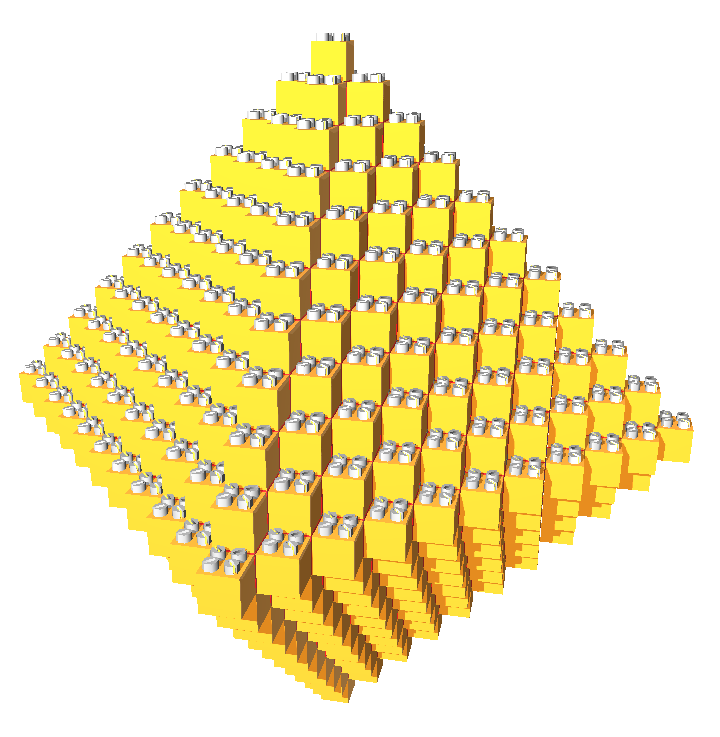
\includegraphics[width=\linewidth]{fig/synchronization/bb-ball-10.png}
  		{\tiny~\\10-hop-radius ball\\\vspace{-1em}1561 Blinky Blocks}
  		\end{column}
  	\end{columns}
  \end{center}
  
\end{frame}
}

\begin{frame} \frametitle{Impact of the Synchronization Period}
  \begin{center}
    \begin{columns}[c]
      \begin{column}{.325\textwidth}
        \centering
        \adjincludegraphics[width=\linewidth,valign=t]{fig/synchronization/L-green.png}\\
        {
        \small
        Duration: 1 hour\\
        Window size: 5
      	}
      \end{column}
      \begin{column}{.675\textwidth}
        \centering
        \adjincludegraphics[width=\linewidth,valign=t]{fig/synchronization/period-hw.pdf}
      \end{column}
  \end{columns}
  \end{center}
  \vfill
  \begin{center}
    \remark{MRTP keeps the system synchronized to a few milliseconds even with a synchronization period of 60 seconds}
    \remark{The synchronization period depends on the desired precision. A long period uses less system resources.}
  \end{center}
\end{frame}

\subsubsection{Simulation Fidelity}

\noLogo{
\begin{frame} \frametitle{VisibleSim Simulator Fidelity}

\begin{center}
	\begin{columns}[c]
		\begin{column}{.35\textwidth}
		Statistical models:
		\begin{itemize}
			\item Clock
				\begin{itemize}
					\item Skew
					\item Drift
					\item Noise (replayed)
				\end{itemize}
			\item Communication time
			\item Processing time
		\end{itemize}
	
		\begin{center}
		\remark{Accurate simulation}
		\end{center}
	
		\end{column}
		\begin{column}{.65\textwidth}
			\footnotesize
			\centering
			Global time dissemination error
			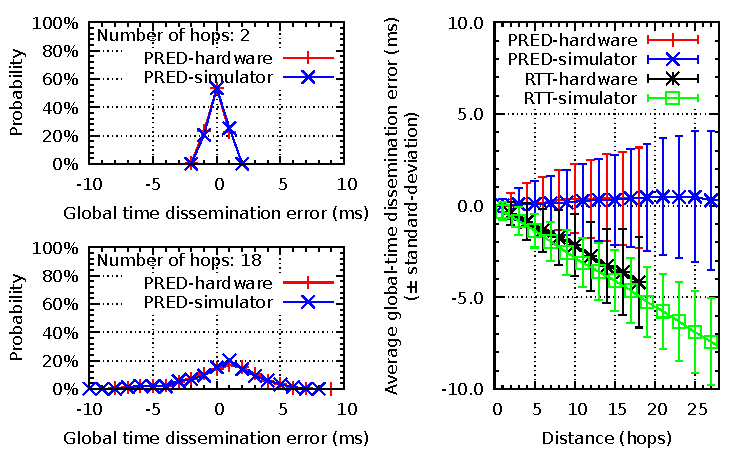
\includegraphics[width=0.75\linewidth]{fig/synchronization/dissemination-error-sim}\\
			Synchronization precision
			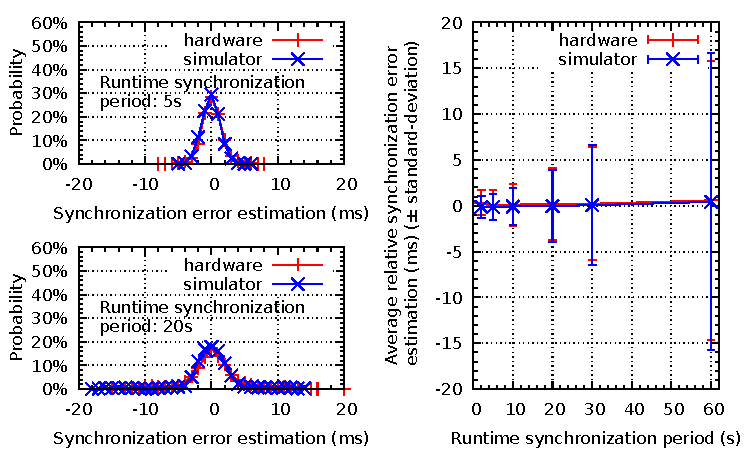
\includegraphics[width=0.75\linewidth]{fig/synchronization/period}
		\end{column}
	\end{columns}
\end{center}
\end{frame}
}

\subsubsection{Simulation Results}

\begin{frame} \frametitle{Simulation Evaluation}

\begin{itemize}
	\item Simulations using VisibleSim
	\item Comparisons with ported version of existing protocols
	\begin{itemize}
		%~\cite{schenato2011average}
		\item Decentralized: ATS [Schenato et al., 2011], WMTS \cite{he2014study} 
		\item Master/Slave with tree: TPSN + MLE \cite{leng2010clock}
		\item Master/Slave but infrastructureless: PulseSync \cite{lenzen2015pulsesync}
	\end{itemize}
	\item Experiments:
	\begin{itemize}
		\item Ball systems (octahedrally-shaped)
		\begin{itemize}
			\item Size: 231 to 27,775 modules
			\item Diameter: 10 to 54 hops
		\end{itemize}
		\item Scenario:
			\begin{itemize}
				\item Left unsynchronized for 1 hour
				\item Then synchronization every 5 seconds during 1 hour
				\item Measurements the maximum pairwise synchronization error every 3 seconds
			\end{itemize}
	\end{itemize}
	\item Evaluation criteria
	\begin{itemize}
		\item Time of convergence
		\item Synchronization precision
		\item Messages
	\end{itemize}
\end{itemize}
\end{frame}

\begin{frame} \frametitle{Convergence Time}

\begin{center}
	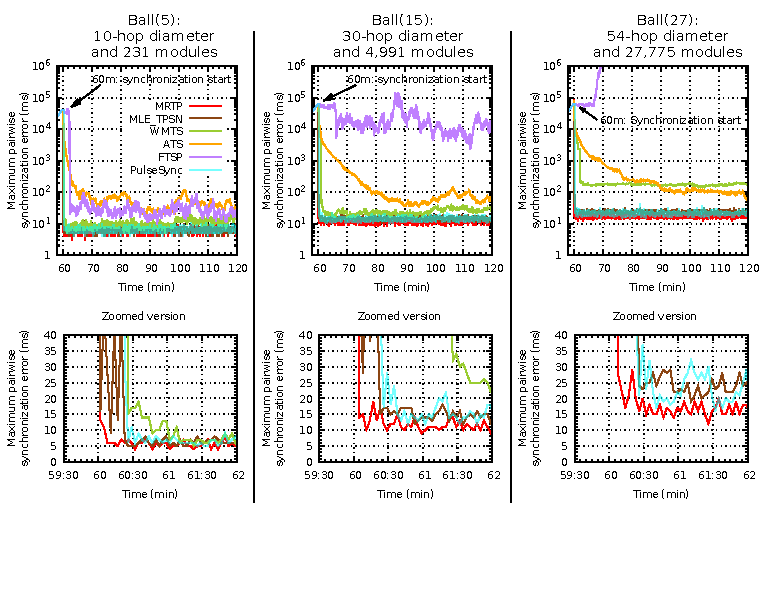
\includegraphics[width=0.9\linewidth]{fig/synchronization/error-time-all-3x2}
\end{center}

\vspace{-1.5cm}
\remark{MRTP converges quickly}

\end{frame}

\begin{frame} \frametitle{Synchronization Precision after Convergence}

\begin{center}
	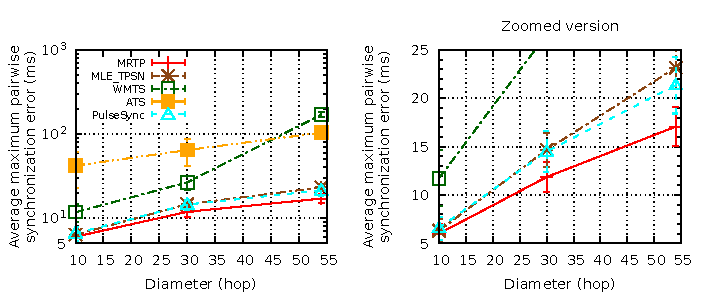
\includegraphics[width=0.9\linewidth]{fig/synchronization/precision}
\end{center}

\remark{MRTP is the most precise protocol}

\remark{MRTP synchronizes the 27,775 module system to 17ms in average}

\end{frame}

\begin{frame} \frametitle{Messages}

\begin{center}
	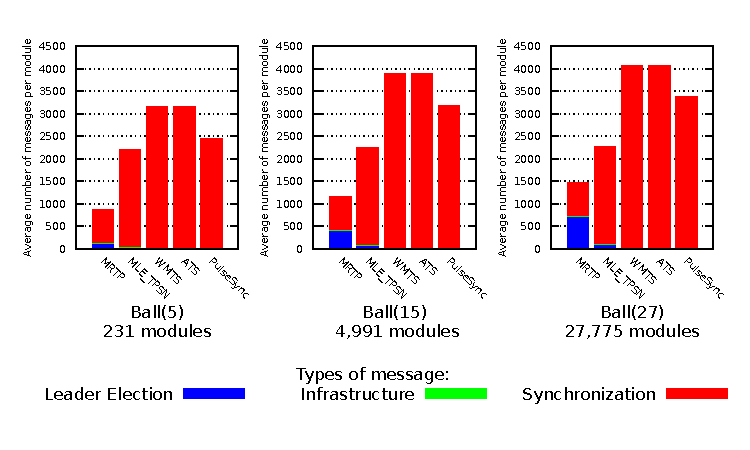
\includegraphics[width=0.9\linewidth]{fig/synchronization/messages}
\end{center}

\remark{MRTP uses few messages}

\end{frame}

\subsection{Conclusion}

\begin{frame} \frametitle{Conclusion}

\begin{itemize}
	\item The Modular Robot Time Protocol (MRTP)
	\item Evaluation
	\begin{itemize}
		\item Hardware
		\item Simulations
		\begin{itemize}
			\item Most precise protocol with a fast convergence
			\item Synchronizes a 27,775 module system with a 54-hop diameter to $< 20ms$ 
			\item Uses less messages in compact systems than existing algorithms
		\end{itemize}
	\end{itemize}
	\item Limit
	\begin{itemize}
		\item Targets fairly stable systems
	\end{itemize}
\end{itemize}
\end{frame}